\begin{figure}
	\centering
	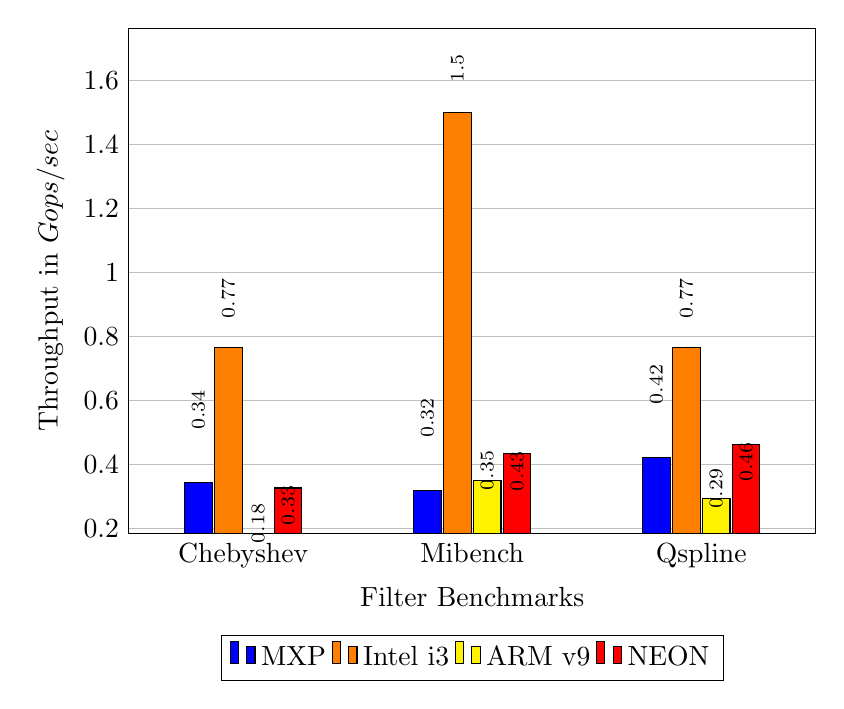
\begin{tikzpicture}
	\begin{axis}[
	width  = 0.85*\textwidth,
	height = 8cm,
	major x tick style = transparent,
	bar width=10pt,
	ymajorgrids = true,
	ylabel = {Throughput in $Gops/sec$},
	xlabel = {Filter Benchmarks},
	symbolic x coords={Chebyshev,Mibench,Qspline},
	major tick length=0cm,
	xtick = data,
	nodes near coords,
	ybar,
	every node near coord/.append style={rotate=90, anchor=west,font=\scriptsize, xshift=0.25cm},
	scaled y ticks = false,
	enlarge y limits={upper,value=0.2},
	enlarge x limits=0.25,
	ybar=2*\pgflinewidth,
	legend cell align=left,
	legend style={
	at={(.5,-0.2)},
	anchor=north,
	legend columns=-1
	column sep=0.5ex
}
	]
	\addplot[draw=black,fill=blue,every node near coord/.append style={xshift=.3cm}]
	coordinates {(Chebyshev, 0.342) (Mibench,0.317) (Qspline,0.422)};
	
	\addplot[draw=black,fill=orange]
	coordinates {(Chebyshev, 0.7651) (Mibench,1.50) (Qspline,0.7651)};
	
	\addplot[draw=black,fill=yellow, every node near coord/.append style={xshift=-0.5cm}]
	coordinates {(Chebyshev, 0.1835) (Mibench,0.3495) (Qspline,0.2941)};
	
	\addplot[draw=black,fill=red, every node near coord/.append style={xshift=-.85cm}]
	coordinates {(Chebyshev, 0.326) (Mibench,0.4338) (Qspline,0.4622)};
	
	\legend{MXP,Intel i3,ARM v9,NEON}
	\end{axis}
	\end{tikzpicture}
	\caption{Word(32-bits) level throughput(Gops/sec) for filter benchmarks }
	\label{fil:3}
\end{figure}